% conformal_interval_width.tex - Histogram comparing interval widths across methods
% TODO: Update with actual validation results when available

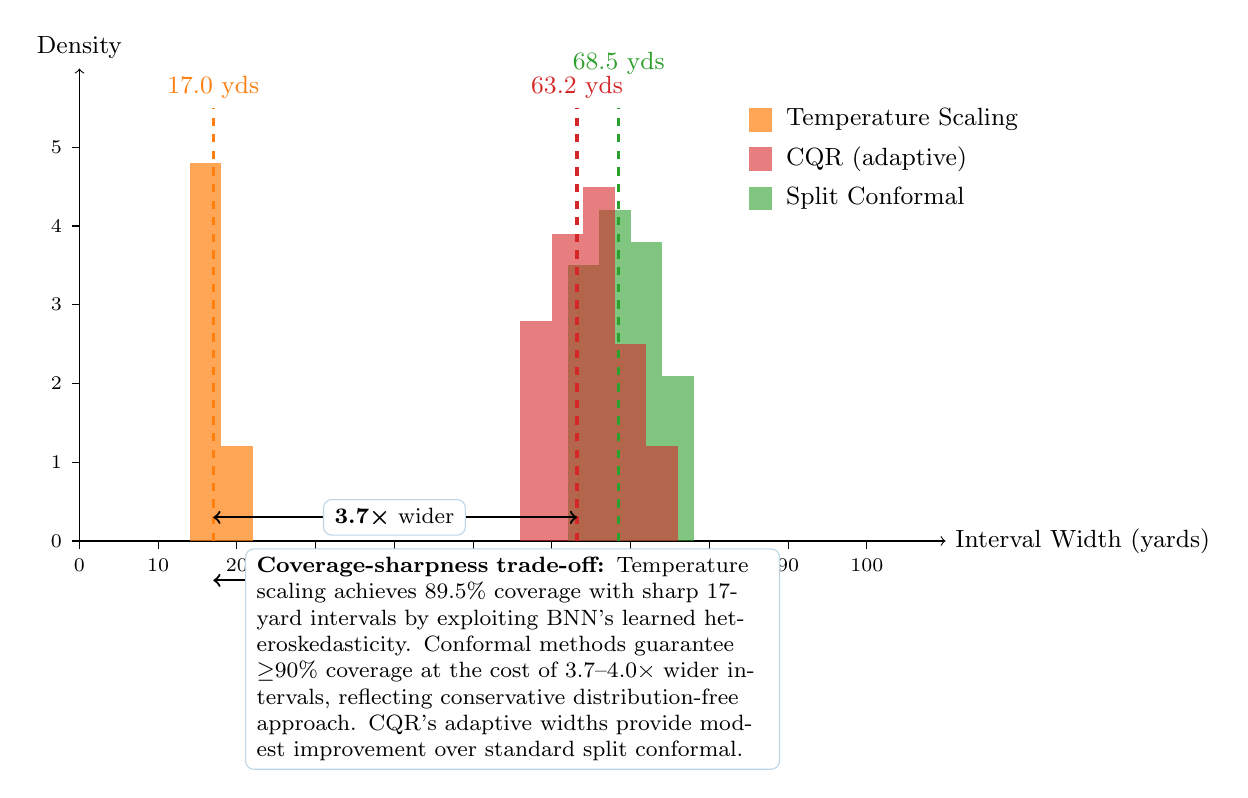
\begin{tikzpicture}
  % Load standardized styles
  % tikz_diagram_style.tex - Standardized TikZ diagram styling
% Updated: January 2026 - Publication-ready minimum sizes

% Define accent color (always set to ensure consistency)
\providecolor{accent}{RGB}{31,119,180}

% ---------------------------------------------------
% MINIMUM SIZE STANDARDS (for legibility)
% ---------------------------------------------------
% - Node text: minimum 9pt (\small or \footnotesize)
% - Arrow labels: minimum 8pt (\footnotesize)
% - Box width: minimum 2.5cm for readable text
% - Inner padding: minimum 6pt vertical, 8pt horizontal

% ---------------------------------------------------
% FLOWCHART STYLES
% ---------------------------------------------------

% Standard flowchart box - readable text with adequate padding
\tikzstyle{flowbox}=[
  draw=accent!60,
  rounded corners=4pt,
  line width=0.6pt,
  fill=accent!5,
  text width=3.2cm,           % Increased from 3cm
  minimum height=1.2cm,       % Ensure minimum height
  align=center,
  font=\small,                % Explicit 10pt minimum
  inner ysep=8pt,             % Increased from 6pt
  inner xsep=10pt             % Increased from 8pt
]

% Wide flowbox for longer text (full width)
\tikzstyle{flowbox-wide}=[
  flowbox,
  text width=0.84\linewidth
]

% Narrow flowbox for compact diagrams
\tikzstyle{flowbox-narrow}=[
  flowbox,
  text width=2.5cm,
  font=\footnotesize          % 9pt for narrow boxes
]

% Large flowbox for main components in architecture diagrams
\tikzstyle{flowbox-large}=[
  flowbox,
  text width=4.5cm,
  minimum height=1.5cm,
  font=\normalsize            % 12pt for emphasis
]

% ---------------------------------------------------
% ARROW STYLES
% ---------------------------------------------------

% Standard directional arrow
\tikzstyle{arrow}=[
  ->,
  >=Stealth,                  % Better arrowhead
  line width=0.7pt,           % Slightly thicker for visibility
  color=accent
]

% Thick arrow for emphasis
\tikzstyle{arrow-thick}=[
  arrow,
  line width=1.2pt
]

% Dashed arrow for optional/secondary flows
\tikzstyle{arrow-dashed}=[
  arrow,
  dashed
]

% Bidirectional arrow
\tikzstyle{arrow-bidir}=[
  <->,
  >=Stealth,
  line width=0.7pt,
  color=accent
]

% ---------------------------------------------------
% LABEL AND ANNOTATION STYLES
% ---------------------------------------------------

% Note/callout style - readable annotation
\tikzstyle{note}=[
  font=\footnotesize,         % Increased from \scriptsize (8pt minimum)
  text=black,
  fill=white,
  draw=accent!30,
  rounded corners=3pt,
  inner xsep=4pt,             % Increased from 2pt
  inner ysep=3pt,             % Increased from 1pt
  align=center
]

% Edge label style for arrow annotations
\tikzstyle{edgelabel}=[
  font=\footnotesize,         % 9pt minimum for edge labels
  fill=white,
  inner sep=2pt
]

% ---------------------------------------------------
% ICON AND MARKER STYLES
% ---------------------------------------------------

% Icon circle style
\tikzstyle{icon}=[
  draw=none,
  circle,
  fill=accent!25,
  minimum size=16pt,          % Increased from 13pt
  inner sep=0pt,
  font=\footnotesize\bfseries % Increased from \scriptsize
]

% Numbered step circle
\tikzstyle{stepnum}=[
  circle,
  draw=accent,
  fill=white,
  minimum size=18pt,
  inner sep=0pt,
  font=\footnotesize\bfseries
]

% ---------------------------------------------------
% ARCHITECTURE DIAGRAM STYLES
% ---------------------------------------------------

% Component box for system architecture
\tikzstyle{component}=[
  draw=accent!70,
  rounded corners=6pt,
  line width=0.8pt,
  fill=accent!8,
  text width=4cm,
  minimum height=1.8cm,
  align=center,
  font=\small\bfseries,
  inner sep=10pt
]

% Subcomponent box (nested inside components)
\tikzstyle{subcomponent}=[
  draw=grey5,
  rounded corners=3pt,
  line width=0.5pt,
  fill=white,
  text width=3cm,
  minimum height=1cm,
  align=center,
  font=\footnotesize,
  inner sep=6pt
]

% Database cylinder style
\tikzstyle{database}=[
  cylinder,
  cylinder uses custom fill,
  cylinder body fill=accent!10,
  cylinder end fill=accent!20,
  draw=accent!60,
  minimum width=2cm,
  minimum height=1.5cm,
  font=\small,
  align=center
]

% Cloud/external service style
\tikzstyle{cloud}=[
  draw=grey5,
  fill=grey7!30,
  rounded corners=8pt,
  text width=3cm,
  minimum height=1.2cm,
  align=center,
  font=\small,
  inner sep=8pt
]

% ---------------------------------------------------
% GROUPING AND CONTAINER STYLES
% ---------------------------------------------------

% Container box for grouping related elements
\tikzstyle{container}=[
  draw=grey5,
  dashed,
  rounded corners=6pt,
  line width=0.6pt,
  fill=none,
  inner sep=12pt
]

% Container label
\tikzstyle{containerlabel}=[
  font=\footnotesize\itshape,
  text=grey3,
  anchor=north west
]


  % Define colors
  \definecolor{accent}{RGB}{31,119,180}
  \definecolor{tempcolor}{RGB}{255,127,14}  % Orange
  \definecolor{conformalcolor}{RGB}{44,160,44}  % Green
  \definecolor{cqrcolor}{RGB}{214,39,40}  % Red

  % Axes
  \draw[->] (0,0) -- (11,0) node[right, font=\small] {Interval Width (yards)};
  \draw[->] (0,0) -- (0,6) node[above, font=\small] {Density};

  % Histogram bars (placeholder data - TODO: replace with actual results)

  % Temperature Scaling (narrow, centered at 17 yards)
  \fill[tempcolor, opacity=0.7] (1.4,0) rectangle (1.8,4.8);
  \fill[tempcolor, opacity=0.7] (1.8,0) rectangle (2.2,1.2);

  % Conformal (BNN base) (wide, centered at 68.5 yards)
  \fill[conformalcolor, opacity=0.6] (6.2,0) rectangle (6.6,3.5);
  \fill[conformalcolor, opacity=0.6] (6.6,0) rectangle (7.0,4.2);
  \fill[conformalcolor, opacity=0.6] (7.0,0) rectangle (7.4,3.8);
  \fill[conformalcolor, opacity=0.6] (7.4,0) rectangle (7.8,2.1);

  % CQR (slightly narrower than standard conformal, centered at 63.2 yards)
  \fill[cqrcolor, opacity=0.6] (5.6,0) rectangle (6.0,2.8);
  \fill[cqrcolor, opacity=0.6] (6.0,0) rectangle (6.4,3.9);
  \fill[cqrcolor, opacity=0.6] (6.4,0) rectangle (6.8,4.5);
  \fill[cqrcolor, opacity=0.6] (6.8,0) rectangle (7.2,2.5);
  \fill[cqrcolor, opacity=0.6] (7.2,0) rectangle (7.6,1.2);

  % Axis ticks and labels
  \foreach \x in {0,10,20,...,100} {
    \pgfmathsetmacro{\xpos}{\x/10}
    \draw (\xpos, -0.1) -- (\xpos, 0);
    \node[below, font=\scriptsize] at (\xpos, -0.1) {\x};
  }

  \foreach \y in {0,1,...,5} {
    \draw (-0.1, \y) -- (0, \y);
    \node[left, font=\scriptsize] at (-0.1, \y) {\y};
  }

  % Mean markers
  \draw[tempcolor, very thick, dashed] (1.7,0) -- (1.7,5.5);
  \node[tempcolor, font=\small, above] at (1.7, 5.5) {17.0 yds};

  \draw[cqrcolor, very thick, dashed] (6.32,0) -- (6.32,5.5);
  \node[cqrcolor, font=\small, above] at (6.32, 5.5) {63.2 yds};

  \draw[conformalcolor, very thick, dashed] (6.85,0) -- (6.85,5.5);
  \node[conformalcolor, font=\small, above] at (6.85, 5.8) {68.5 yds};

  % Sharpness comparison annotations
  \draw[<->, thick, black] (1.7, 0.3) -- (6.32, 0.3);
  \node[note, fill=white] at (4.0, 0.3) {\textbf{3.7×} wider};

  \draw[<->, thick, black] (1.7, -0.5) -- (6.85, -0.5);
  \node[note, fill=white] at (4.3, -0.5) {\textbf{4.0×} wider};

  % Legend
  \fill[tempcolor, opacity=0.7] (8.5, 5.2) rectangle (8.8, 5.5);
  \node[right, font=\small] at (8.85, 5.35) {Temperature Scaling};

  \fill[cqrcolor, opacity=0.6] (8.5, 4.7) rectangle (8.8, 5.0);
  \node[right, font=\small] at (8.85, 4.85) {CQR (adaptive)};

  \fill[conformalcolor, opacity=0.6] (8.5, 4.2) rectangle (8.8, 4.5);
  \node[right, font=\small] at (8.85, 4.35) {Split Conformal};

  % Note
  \node[note, text width=6.5cm, align=left] at (5.5, -1.5) {
    \textbf{Coverage-sharpness trade-off:} Temperature scaling achieves 89.5\% coverage
    with sharp 17-yard intervals by exploiting BNN's learned heteroskedasticity.
    Conformal methods guarantee $\geq$90\% coverage at the cost of 3.7--4.0× wider intervals,
    reflecting conservative distribution-free approach. CQR's adaptive widths provide modest
    improvement over standard split conformal.
  };

\end{tikzpicture}
